
\documentclass[template=tabling,81pt,headonall]{azmoon}
\usepackage{xepersian}
\usepackage{amsfonts}
\usepackage{graphicx}
\usepackage{svg}
\svgpath{ {./images/} }
\graphicspath{ {./images/} }
\settextfont{Yas}
\setdigitfont{A Iranian Sans}
\usepackage{fontawesome5}

\printanswers
    \teacher{محمد صالح علی اکبری}
    \teachertitle{دبیر}
    \city{گناباد}
    \schooltitle{متوسطه دوره اول}
    \school{شهید دکتر چمران}
    \grade{دهم}
    \branch{101}
    \topic{ریاضی}
    \examdate{۱۲/۱۲/۱۴۰۳}
    \answertime{۵۰ دقیقه}
    \begin{document}
	\begin{questions}
		\nointerlineskip%
		\vskip-\baselineskip
		\question[0.5]{%
کدام یک نمودار معادله خط $y = 3x-2$ را نشان می‌دهد؟
    \begin{fourchoice}[2]\choice{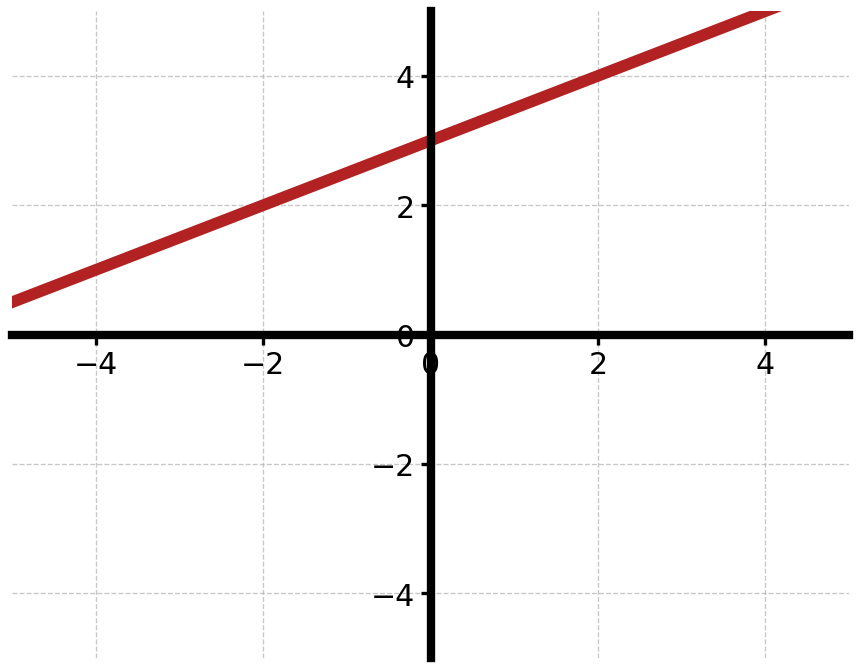
\includegraphics[scale = 0.4]{y__=__0.5x__+__3}}
\choice{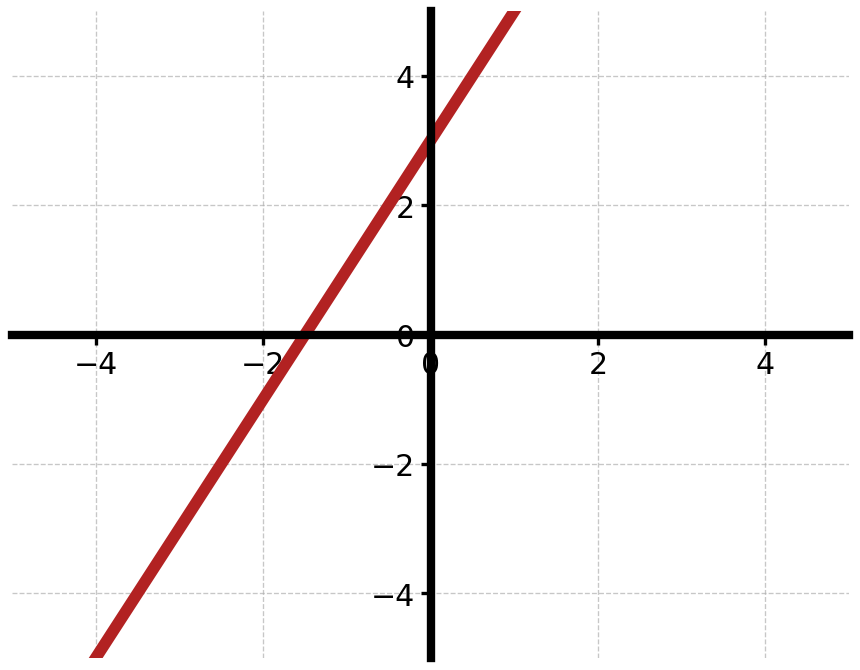
\includegraphics[scale = 0.4]{y__=__2x__+__3}}
\choice{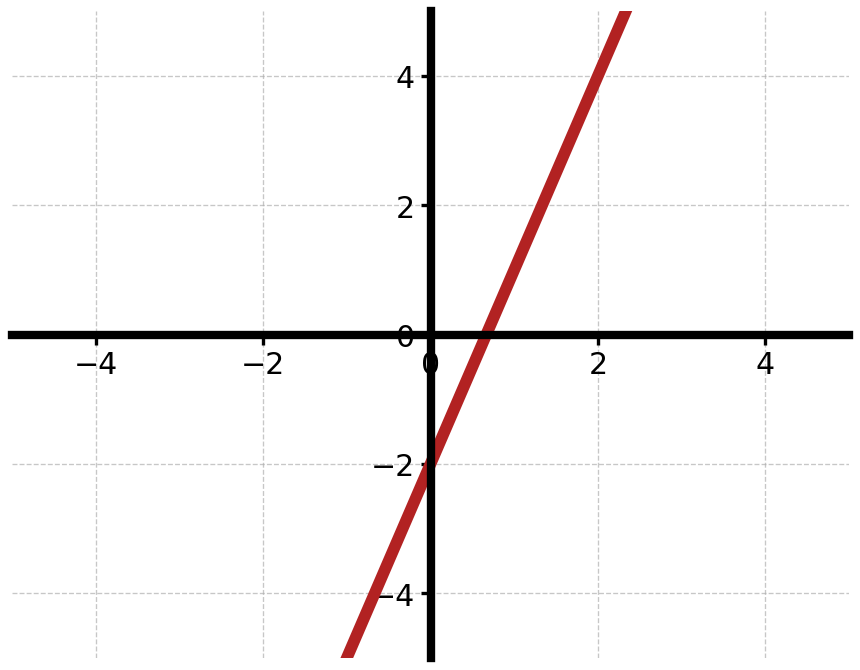
\includegraphics[scale = 0.4]{y__=__3x__+___-_2}}
\choice{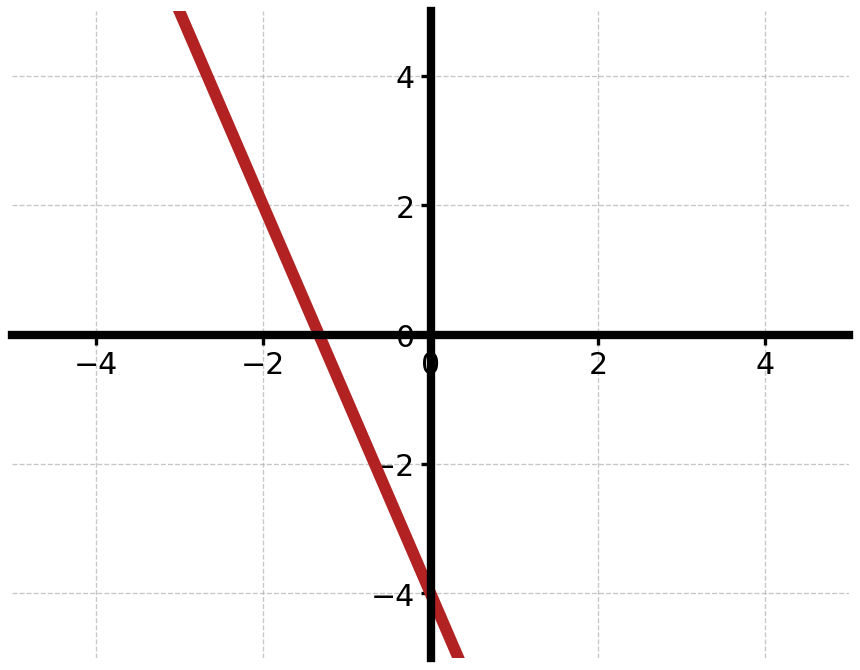
\includegraphics[scale = 0.4]{y__=___-_3x__-__4}}
\end{fourchoice}

            }\question[0.5]{%
این نمودار مربوط به چه معادله خطی است؟
                            \\ 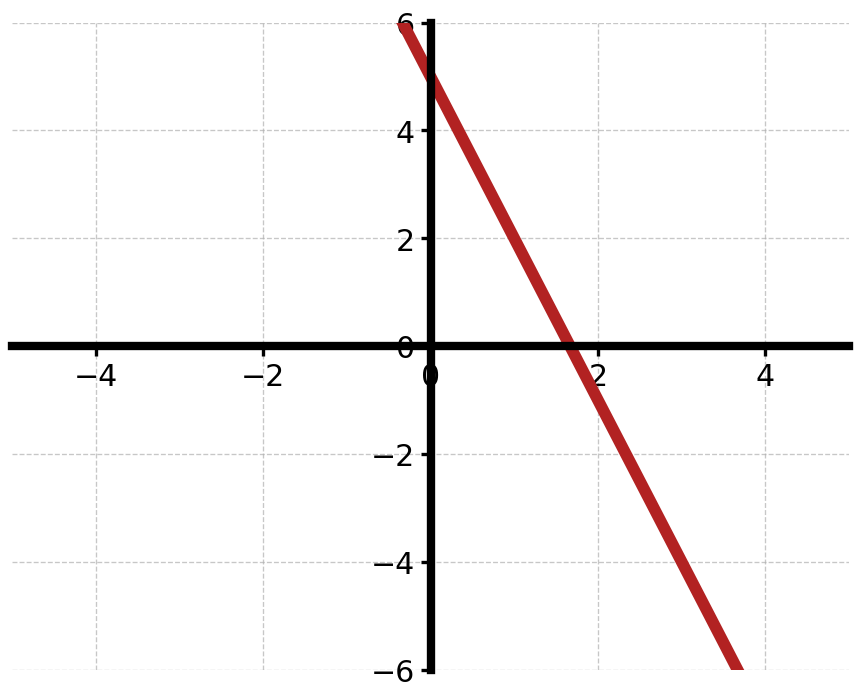
\includegraphics[scale = 0.4]{y__=___-_3x__+__5}
    \begin{fourchoice}[4]\choice{$y = 5x + 3$}
\choice{$y = -3x + 5$}
\choice{$y = -3x - 5$}
\choice{$y = 3x + 5$}
\end{fourchoice}

            }\question[0.5]{%
با قرار دادن کدام یک از گزینه‌های زیر به جای $x$ معادله $3x -7 = \dfrac{5x - 8}{2}$ برقرار می‌شود؟
    \begin{fourchoice}[4]\choice{$4$}
\choice{$6$}
\choice{$8$}
\choice{$12$}
\end{fourchoice}

            }\question[0.5]{%
با قرار دادن کدام یک از گزینه‌های زیر به جای $x$ معادله $x^2 - 10x + 24 = 0$ برقرار می‌شود؟
    \begin{fourchoice}[4]\choice{$4$ و $6$}
\choice{$6$ و $12$}
\choice{$3$ و $4$}
\choice{$8$}
\end{fourchoice}

            }\question[0.5]{%
با قرار دادن کدام یک از گزینه‌های زیر به جای $x$ معادله $x^2 - 8x + 15 = 0$ برقرار می‌شود؟
    \begin{fourchoice}[4]\choice{$2$ و $6$}
\choice{$4$ و $4$}
\choice{$3$ و $5$}
\choice{$8$}
\end{fourchoice}

            }\question[0.5]{%
با قرار دادن کدام یک از گزینه‌های زیر به جای $x$ معادله $x^2 - 5x + 6 = 0$ برقرار می‌شود؟
    \begin{fourchoice}[4]\choice{$1$ و $6$}
\choice{$4$ و $5$}
\choice{$2$ و $3$}
\choice{$5$}
\end{fourchoice}

            }\question[0.5]{%
با قرار دادن کدام یک از گزینه‌های زیر به جای $x$ معادله $x^2 - 7x + 12 = 0$ برقرار می‌شود؟
    \begin{fourchoice}[4]\choice{$3$ و $4$}
\choice{$4$ و $5$}
\choice{$2$ و $6$}
\choice{$7$}
\end{fourchoice}

            }\question[0.5]{%
کدام تصویر مربوط به حل معادله به روش هندسی معادل $3x^2 + x - 6 = 0$ است؟
    \begin{fourchoice}[2]\choice{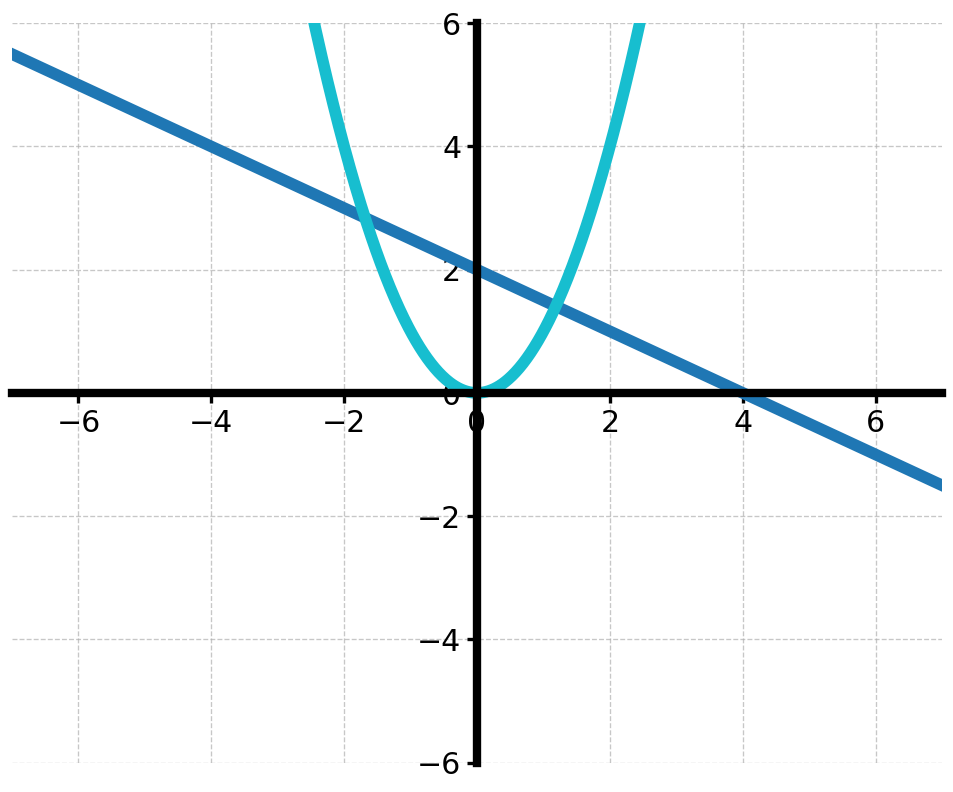
\includegraphics[scale = 0.35]{y__=___-_0.5x_+_2_and_y__=__x_power_2}}
\choice{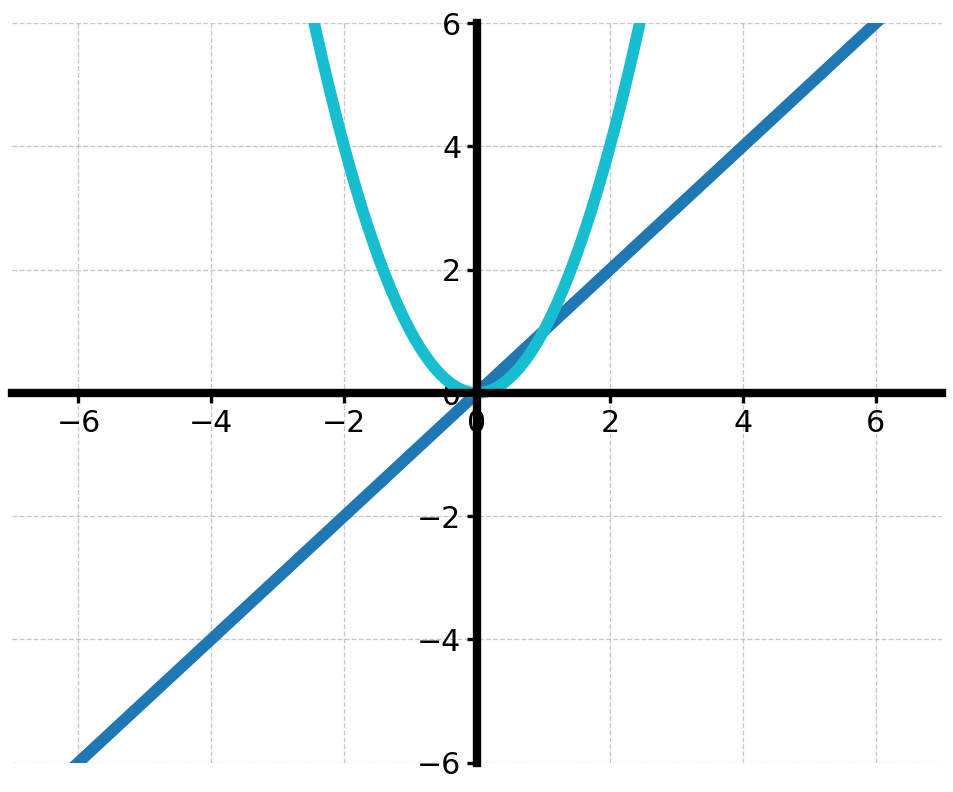
\includegraphics[scale = 0.35]{y__=__1x_and_y__=__x_power_2}}
\choice{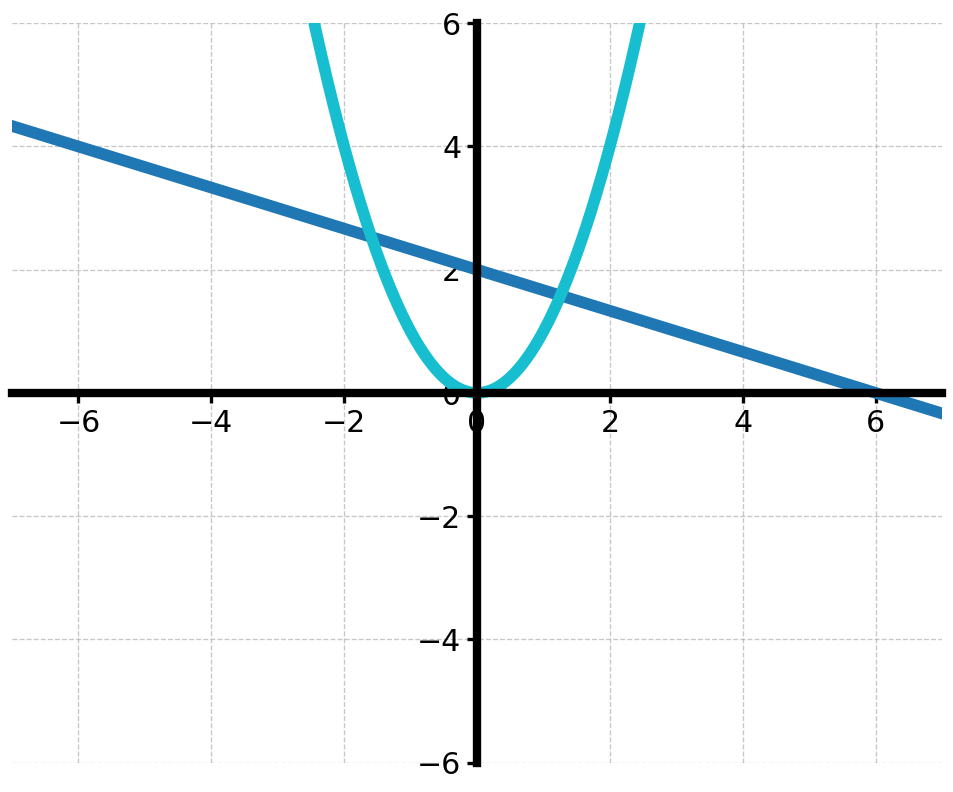
\includegraphics[scale = 0.35]{y__=___-_0.3333x__+__2_and_y__=__x_power_2}}
\choice{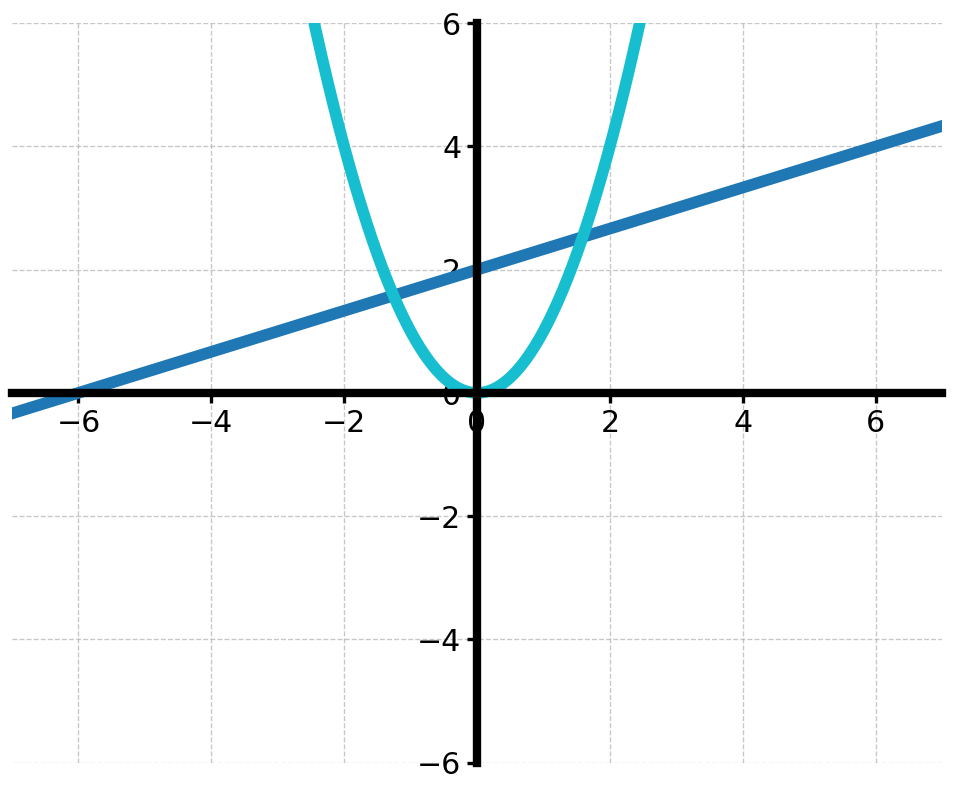
\includegraphics[scale = 0.35]{y__=___+_0.3333x__+__2_and_y__=__x_power_2}}
\end{fourchoice}

            }\question[0.5]{%
کدام تصویر مربوط به حل معادله به روش هندسی معادل $4x^2 + x + 7 = -1$ است؟
    \begin{fourchoice}[2]\choice{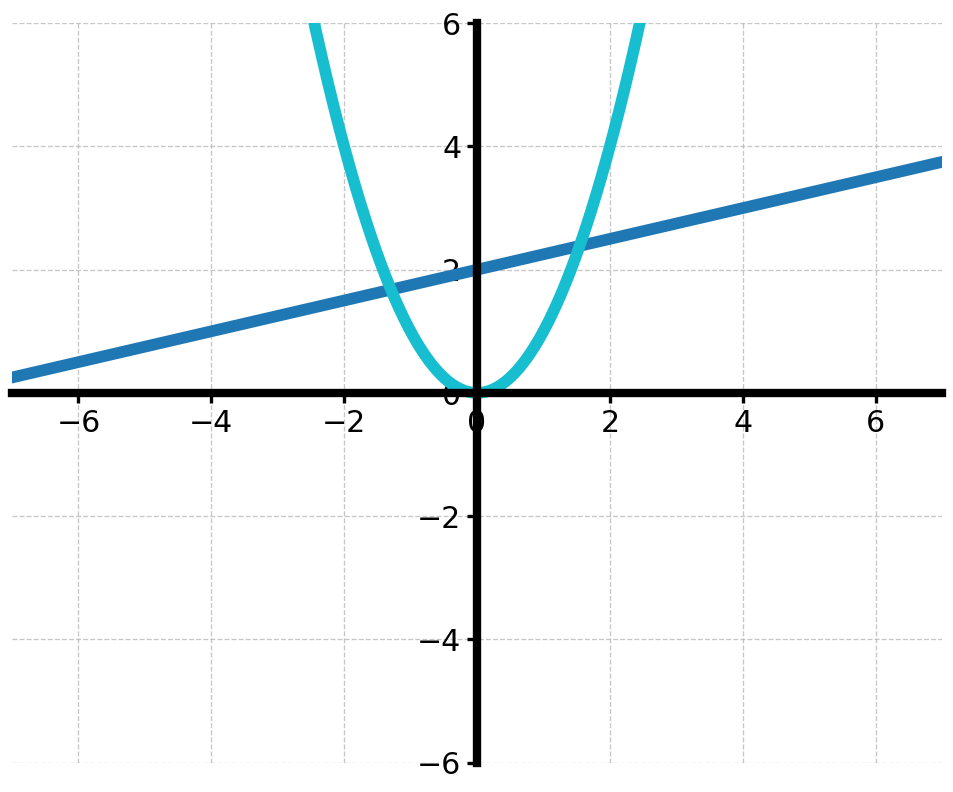
\includegraphics[scale = 0.38]{y__=___+_0.25x__+__2_and_y__=__x_power_2}}
\choice{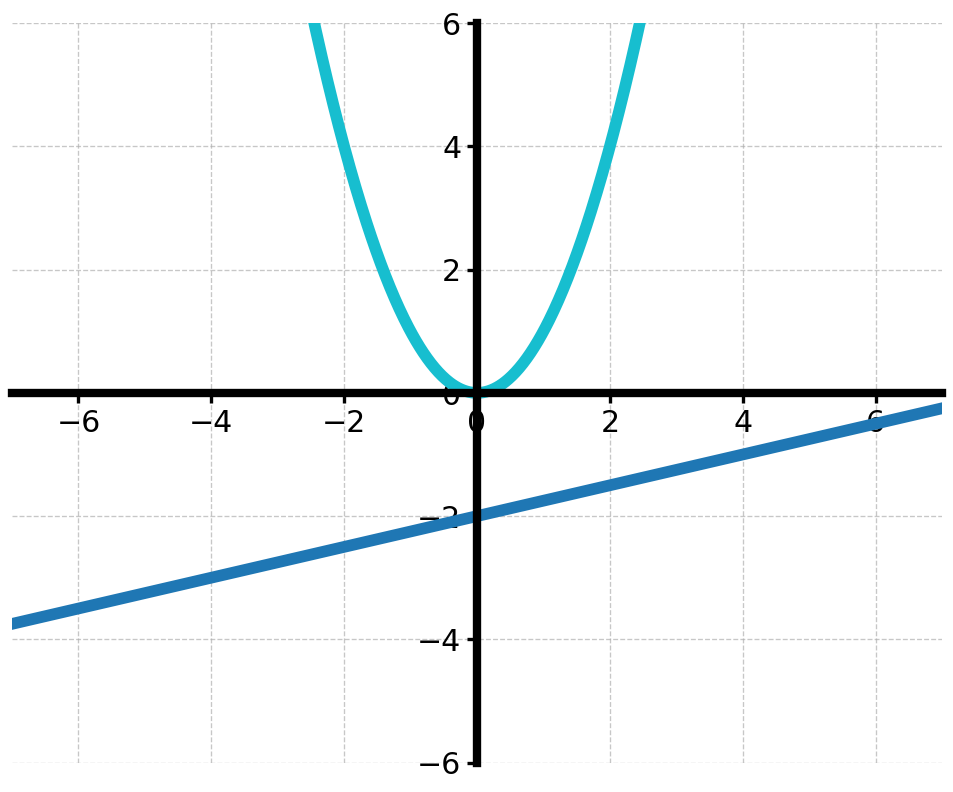
\includegraphics[scale = 0.38]{y__=___+_0.25x__+___-_2_and_y__=__x_power_2}}
\choice{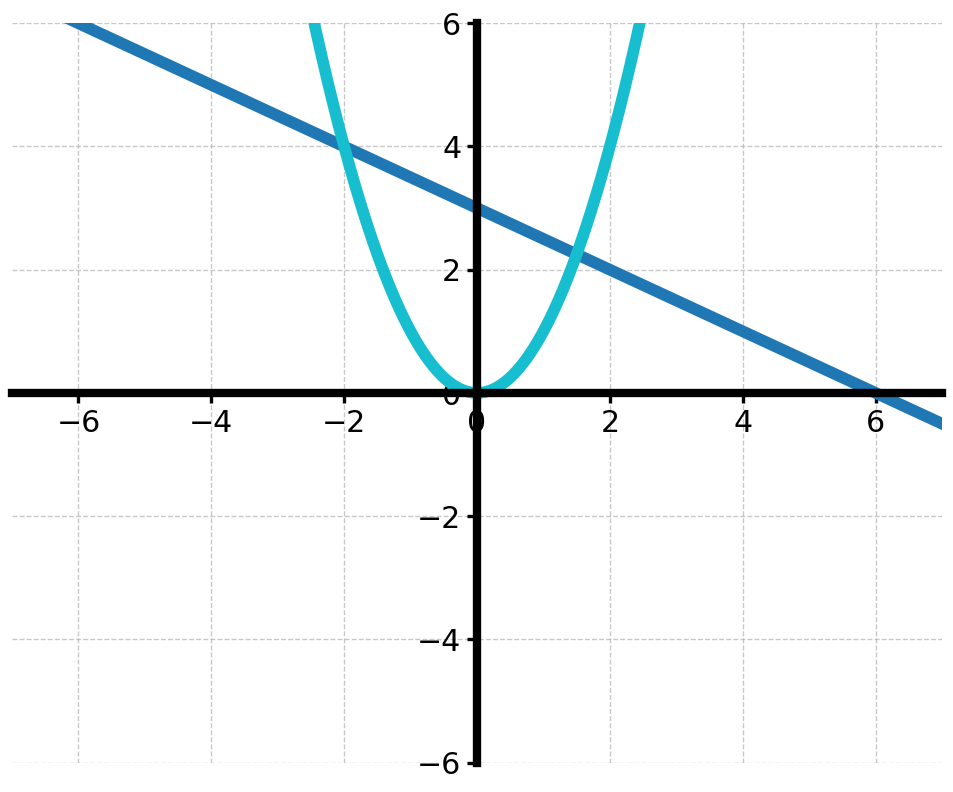
\includegraphics[scale = 0.38]{y__=___-_0.5x_+_3_and_y__=__x_power_2}}
\choice{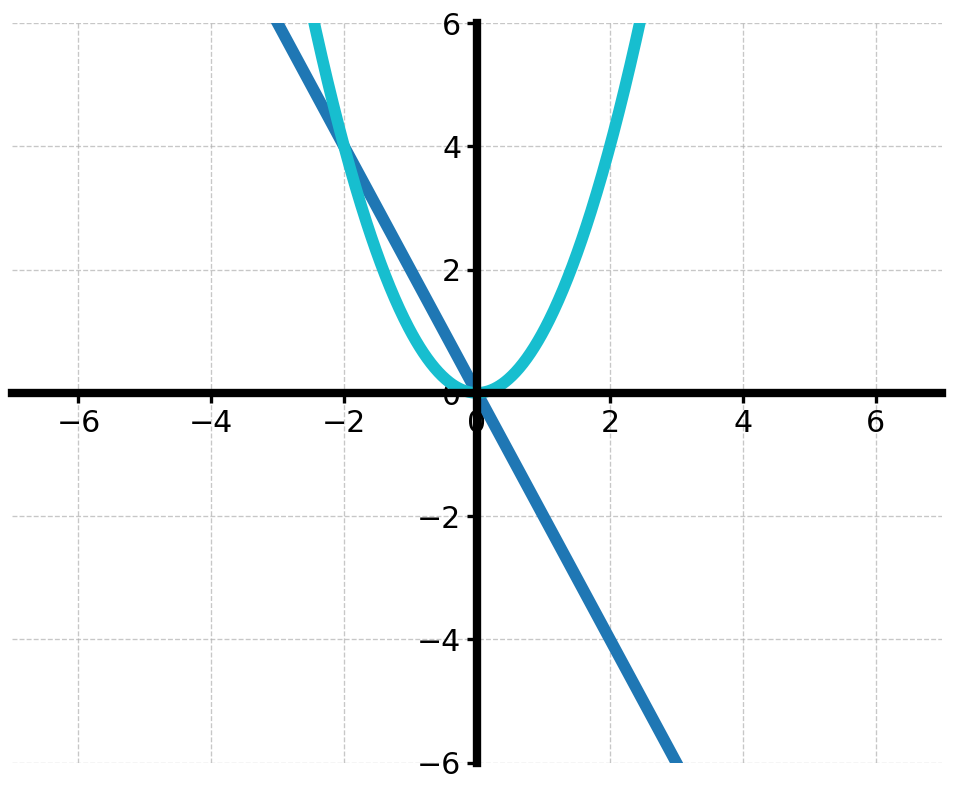
\includegraphics[scale = 0.38]{y__=___-_2x_and_y__=__x_power_2}}
\end{fourchoice}

            }\question[0.5]{%
جواب‌های معادله $x^2 - 6 = 0$ در کدام گزینه وجود دارد؟.
    \begin{fourchoice}[4]\choice{$\sqrt{6}$ و $\sqrt{-6}$}
\choice{$\sqrt{6}$ و $-\sqrt{6}$}
\choice{$\sqrt{-36}$ و $\sqrt{36}$}
\choice{$\sqrt{0}$ و $\sqrt{36}$}
\end{fourchoice}

            }\question[1.5]{%
معادله $x^2 -2x = 0$ را به کمک روش هندسی حل کنید.‌
\\‌
\\‌
\\}\question[1.5]{%
حاصل ضرب دو عدد متوالی $132$ می‌باشد. این دو عدد را پیدا کنید. (راه حل با حل معادله درجه دو) راهنمایی: عدد کوچک تر را $x$ در نظر بگیرید و عدد بزرگ تر را $x+1$ در نظر بگیرید.‌
\\‌
\\‌
\\}\question[2]{%
اگر طول مستطیلی سه برابر عرض آن باشد و مساحت آن 300 متر مربع باشد، طول و عرض این مستطیل چقدر است؟ این مسئله چند جواب دارد؟ ‌
\\‌
\\‌
\\‌
\\}\question[2]{%
اگر جمع دو عدد 20 و ضرب آنها 106 باشد، این دو عدد چه اعدادی هستند؟‌
\\‌
\\‌
\\‌
\\}\question[2]{%
اگر جمع دو عدد -5 و ضرب آنها -14 باشد، این دو عدد چه اعدادی هستند؟‌
\\‌
\\‌
\\‌
\\}\question[2]{%
اگر جمع دو عدد 7 و ضرب آنها 10 باشد، این دو عدد چه اعدادی هستند؟‌
\\‌
\\‌
\\‌
\\}\question[2]{%
اگر جمع دو عدد -3 و ضرب آنها 2 باشد، این دو عدد چه اعدادی هستند؟‌
\\‌
\\‌
\\‌
\\}\end{questions}
    \end{document}
    